% A concave boundary is shortened by replacing its inward detour with a chord.
% Regenerate from this directory:
% latex -interaction=nonstopmode -halt-on-error ch.tex
% dvisvgm --no-fonts --exact --bbox=papersize --output=ch.svg ch.dvi
\documentclass[tikz,border=5pt]{standalone}
\usetikzlibrary{arrows.meta,backgrounds}
\definecolor{boundary}{RGB}{60,112,202}
\definecolor{pointborder}{RGB}{42,75,129}
\begin{document}
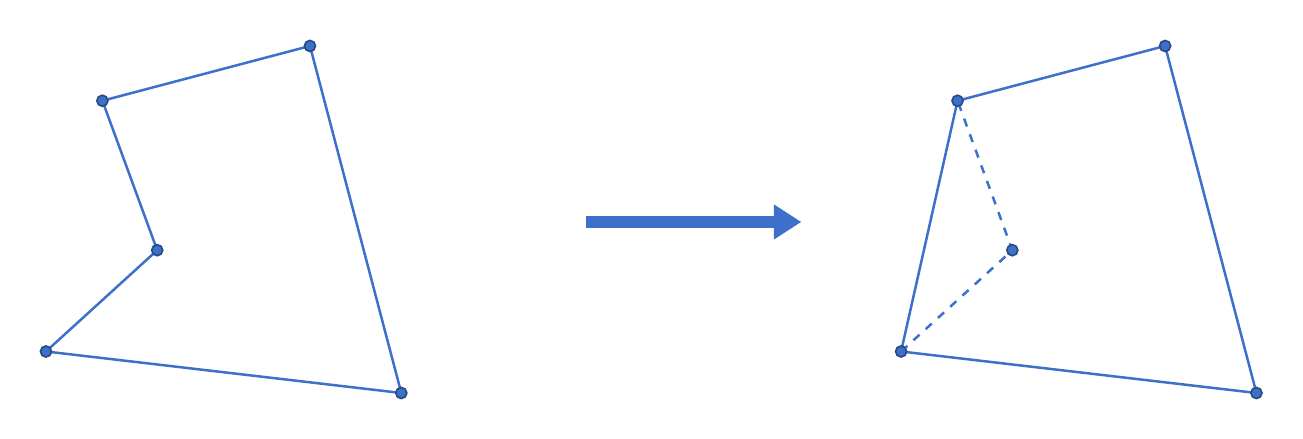
\begin{tikzpicture}[
  x=0.6pt,y=-0.6pt,line width=0.9pt,
  background rectangle/.style={fill=white},show background rectangle
]
  % Both panels contain exactly the same five points. Point B is interior
  % to the convex hull A-C-D-E; A-B-C is the longer, concave detour.
  \foreach \offset in {0,515} {
    \begin{scope}[shift={(\offset,0)}]
      \coordinate (A) at (0,190);
      \coordinate (B) at (67,129);
      \coordinate (C) at (34,39);
      \coordinate (D) at (159,6);
      \coordinate (E) at (214,215);
      \draw[boundary] (C) -- (D) -- (E) -- (A);
      \ifnum\offset=0
        \draw[boundary] (A) -- (B) -- (C);
      \else
        \draw[boundary] (A) -- (C);
        \draw[boundary,dashed] (A) -- (B) -- (C);
      \fi
      \foreach \point in {A,B,C,D,E}
        \filldraw[fill=boundary,draw=pointborder,line width=0.6pt]
          (\point) circle[radius=2pt];
    \end{scope}
  }
  \draw[boundary,line width=4pt,-{Triangle[length=10pt,width=12pt]}]
    (325,112) -- (455,112);
\end{tikzpicture}
\end{document}
